\documentclass[11pt]{beamer}
\usetheme{CambridgeUS}
\usepackage[utf8]{inputenc}
\usepackage{amsmath}
\usepackage{amsfonts}
\usepackage{amssymb}
\usepackage[
backend=biber,
style=alphabetic,
citestyle=authoryear
]{biblatex}

\newcommand\Fontvi{\fontsize{8}{7.2}\selectfont}

% Footnote without number
\newcommand\blfootnote[1]{%
  \begingroup
  \renewcommand\thefootnote{}\footnote{#1}%
  \addtocounter{footnote}{-1}%
  \endgroup
}
\newcommand{\comment}[1]{}

\addbibresource{stats.bib}
\title[Bioestatística II] %optional
{Introdução à Bioestatística}

\subtitle{CGF2046 - Bioestatística II}

\author[da Silva, Ricardo] % (optional, for multiple authors)
{R. ~R. ~da Silva\inst{1}}

\institute[FCFRP] % (optional)
{
  \inst{1}%
  Departamento de Ciências BioMoleculares\\
  Faculdade de Ciências Farmacêuticas

}

\date{\today} % (optional)

\titlegraphic{\includegraphics[width=5.8cm]{figs/logo_final}} 


\begin{document}

\begin{frame}
\titlepage
\end{frame}

\begin{frame}
\label{contents}
\frametitle{Sumário}
\tableofcontents
\end{frame}

\section{Organização da disciplina}
\setbeamercovered{transparent}
\begin{frame}
\frametitle{CGF2022 - Bioestatística I}
Todo material será compartilhado pelo \textit{Google Class Room}:
\\~\\
Código da turma: r6k6ky5l
\\~\\
  \begin{itemize}
  \uncover<1->{\item
    Cronograma de atividades;}
  \uncover<2->{\item
    Capítulos do livro;}
  \uncover<3->{\item
    Discussões de dúvidas e avisos podem ser postados no \textit{Class Room};}
  \uncover<4->{\item
    Dúvidas podem ser enviadas por email: \href{mailto:ridasilva@usp.br}{ridasilva@usp.br}}
  \end{itemize}

\end{frame}

\setbeamercovered{transparent}
\begin{frame}
\frametitle{CGF2022 - Bioestatística I}
Critério de avaliação:
\\~\\
  \begin{itemize}
  \uncover<1->{\item
    \(N = \frac{1 \times E+4.5 \times P1+4.5 \times P2}{10}\), onde \(E=\frac{1}{n}\sum_{i=1}^nN_i\) representa as listas de exercícios, e \(P\) representa as provas 1 e 2;}
  \uncover<2->{\item
    Declaração de Integridade Acadêmica:\\~\\

\textit{"Ao assinar abaixo, nós empenhamos nossa palavra, que as respostas dessa prova foram elaboradas pelo nosso grupo, sem a assistência de pessoas não autorizadas"};}
  \uncover<3->{\item
    Os exercícios devem ser entregues antes da aula de correção;}
  \uncover<4->{\item
    Os exercícios devem ser postados no Class Room, ou enviados por email: \href{mailto:ridasilva@usp.br}{ridasilva@usp.br}, caso haja problemas;}
  \uncover<5->{\item
    Se o aluno obtiver a pontuação mínima para aprovação (5) ou recuperação (3) a presença não será levada em conta. Caso contrário, o estudante será reprovado por faltas.}
  \end{itemize}

\end{frame}

\setbeamercovered{transparent}
\begin{frame}
\frametitle{Perguntas da aula}
  \begin{itemize}
  \item Como podemos resumir os dados na planilha para explicar algo?
  \item Existe diferença entre os dados apresentados em cada coluna?
  \item É possível obter informações confiáveis para dados da coluna da turma com um subconjunto dos dados apresentados da tabela?
  \item Que cuidados você teria para obter informações com um subconjunto?
  \end{itemize}
\end{frame}

\setbeamercovered{transparent}
\begin{frame}
\frametitle{O que é estatística?\footcite{magalhaes2002noccoes}}
Estatística é um conjunto de técnicas para, sistematicamente:
\\~\\
  \begin{itemize}
  \uncover<1->{\item
    Planejar a coleta de dados oriundos de estudos ou experimentos,
    realizados em qualquer área do conhecimento;}
  \uncover<2->{\item
    Descrever, analisar e interpretar dados;}
  \uncover<3->{\item
    Extrair informações para subsidiar decisões;}
  \uncover<4->{\item
    Avaliar evidências empíricas sob hipóteses de interesse.}
  \end{itemize}
\blfootnote{\url{http://www.leg.ufpr.br/}}
\end{frame}

\setbeamercovered{transparent}
\begin{frame}
\frametitle{Descrever, analisar e interpretar dados}

Apresentação: \url{https://www.youtube.com/watch?v=ezVk1ahRF78}\\~\\
Formulário: \url{https://forms.gle/2nQWmvd4chJCKG6NA}

\begin{center}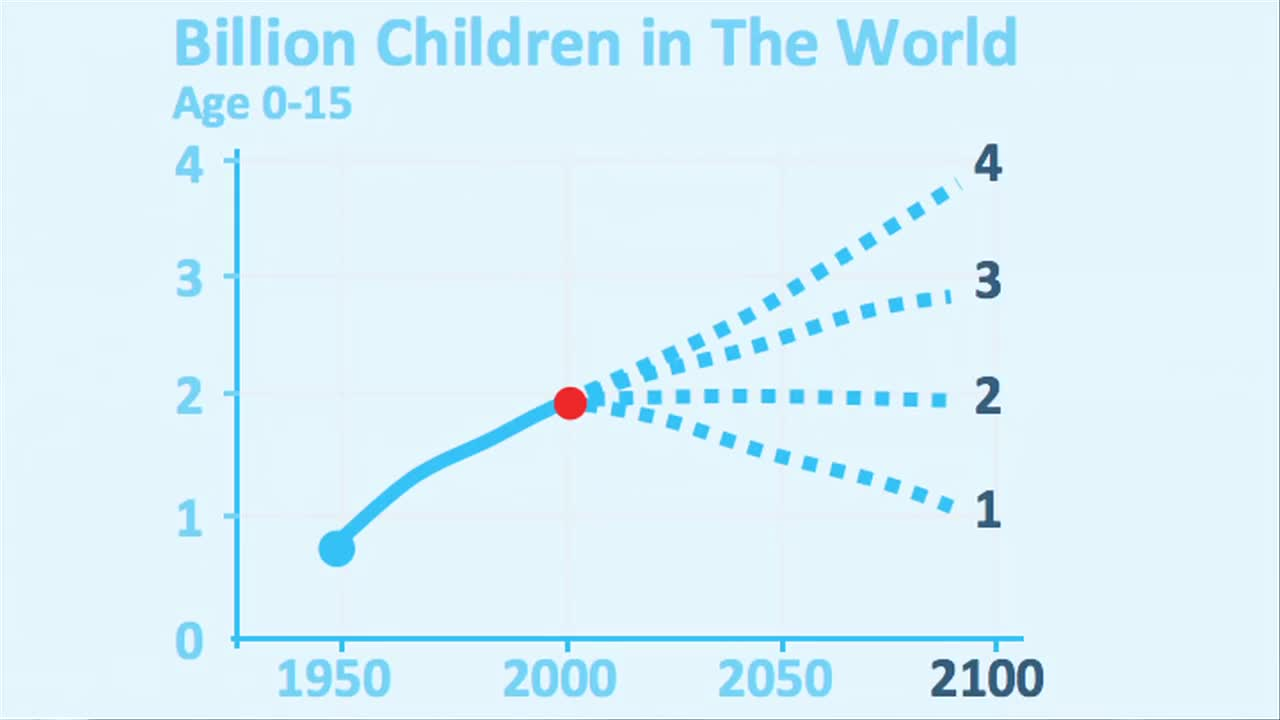
\includegraphics[width=0.9\linewidth]{figs/relegions-and-babies} \end{center}
\end{frame}

% https://www.gapminder.org/videos/religions-and-babies/
% https://www.youtube.com/watch?v=ezVk1ahRF78
% https://pharmchem.cop.ufl.edu/about/articles/what-is-pharmaceutical-chemistry/
% https://www.ime.usp.br/ativestat/
\setbeamercovered{transparent}
\begin{frame}
\frametitle{Utilização opcional de \textit{software}}
O \textit{Colaboratory} pode ser utilizado para fazer os exercícios.

\begin{center}\includegraphics[width=0.5\linewidth]{figs/colab.png} \end{center}

O "Colab" permite que você escreva e execute código (Python) no seu navegador com:
\begin{itemize}
\item Nenhuma configuração requerida;
\item Acesso livre aos GPUs (Unidade de processamento gráfico do seu computador);
\item Facilmente compartilhável.
\end{itemize} 

\blfootnote{\url{colab.research.google.com}}
\end{frame}


\section{Definições básicas}
\setbeamercovered{transparent}
\begin{frame}
\frametitle{O que é estatística?\footcite{magalhaes2002noccoes}}
Estatística é um conjunto de técnicas para, sistematicamente:
\\~\\
  \begin{itemize}
  \uncover<1->{\item
    Planejar a coleta de dados oriundos de estudos ou experimentos,
    realizados em qualquer área do conhecimento;}
  \uncover<2->{\item
    Descrever, analisar e interpretar dados;}
  \uncover<3->{\item
    Extrair informações para subsidiar decisões;}
  \uncover<4->{\item
    Avaliar evidências empíricas sob hipóteses de interesse.}
  \end{itemize}
\blfootnote{\url{http://www.leg.ufpr.br/}}
\end{frame}

\setbeamercovered{transparent}
\begin{frame}
\frametitle{O que é estatística?}
  Exemplos de aplicações:
  \\~\\
  \begin{itemize}
  \uncover<1->{\item
    Opinião da população brasileira sobre o novo governo.}
  \uncover<2->{\item
    Avaliar a efetividade de uma nova droga para a cura do câncer.}
  \uncover<3->{\item
    Entender os hábitos de compra dos clientes de uma loja virtual.}
  \uncover<4->{\item
    Recomendação personalizada de produtos.}
  \uncover<5->{\item
    Comparar a produtividade da soja sob diferentes formas de cultivo,
    adubação, etc.}
  \end{itemize}
\end{frame}

\setbeamercovered{transparent}
\begin{frame}
\frametitle{O que é estatística?}
  Conceitos fundamentais
  \\~\\
  \begin{itemize}
  \uncover<1->{\item
    \textbf{População}: Conjunto de todos os elementos sob investigação.}
  \uncover<2->{\item
    \textbf{Amostra}: Subconjunto da população.}
  \uncover<3->{\item
    \textbf{Variável} de interesse: característica a ser observada em
    cada indivíduo da amostra.}
  \end{itemize}
\end{frame}

\setbeamercovered{transparent}
\begin{frame}
\frametitle{Divisões básicas da estatística}

\begin{center}\includegraphics[width=0.75\linewidth]{figs/populacao_amostra} \end{center}
\blfootnote{\url{http://www.leg.ufpr.br/}}
\end{frame}

\setbeamercovered{transparent}
\begin{frame}
\frametitle{O que é estatística?}
  \Fontvi
  \uncover<1->{
  \textbf{Exemplo 1}: Opinião da população brasileira sobre o novo governo.
    \begin{itemize}
    \item
    \textbf{População}: Todos os habitantes do Brasil? outras opções?
    \item
    \textbf{Amostra}: Algum subconjunto da população. Qualquer um será?
    Como selecionar?
    \item
    \textbf{Variável de interesse}: Opinião sobre o novo governo. Como
    medir isso? Gosta? sim ou não.\\~\\
    \end{itemize}}
  \uncover<2->{
  \textbf{Exemplo 2}: Avaliar a efetividade de uma nova droga para a cura do câncer.  
    \begin{itemize}
    \item
    \textbf{População}: Todos os seres humanos? Apenas os já doentes?
    Como levar em conta questões de raça, culturas, etc \ldots{}
    \item
    \textbf{Amostra}: E agora?
    \item
    \textbf{Variável de interesse}: Curou ou não curou? Será que isso é
    possível? \\~\\
  \end{itemize}}
  \uncover<3->{
  \textbf{Exemplo 3}:
  Entender os hábitos de compra dos clientes de uma loja virtual.
  \begin{itemize}
  \item
    \textbf{População}: Todos os clientes da loja virtual.
  \item
    \textbf{Amostra}: Preciso de amostra?
  \item
    \textbf{Variável de interesse}: E agora? Como caracterizar hábito de
    compra?
  \end{itemize}
  }
\end{frame}


\setbeamercovered{transparent}
\begin{frame}
\frametitle{Desenho de estudos\footcite{martinez2015bioestatistica}}
\begin{center}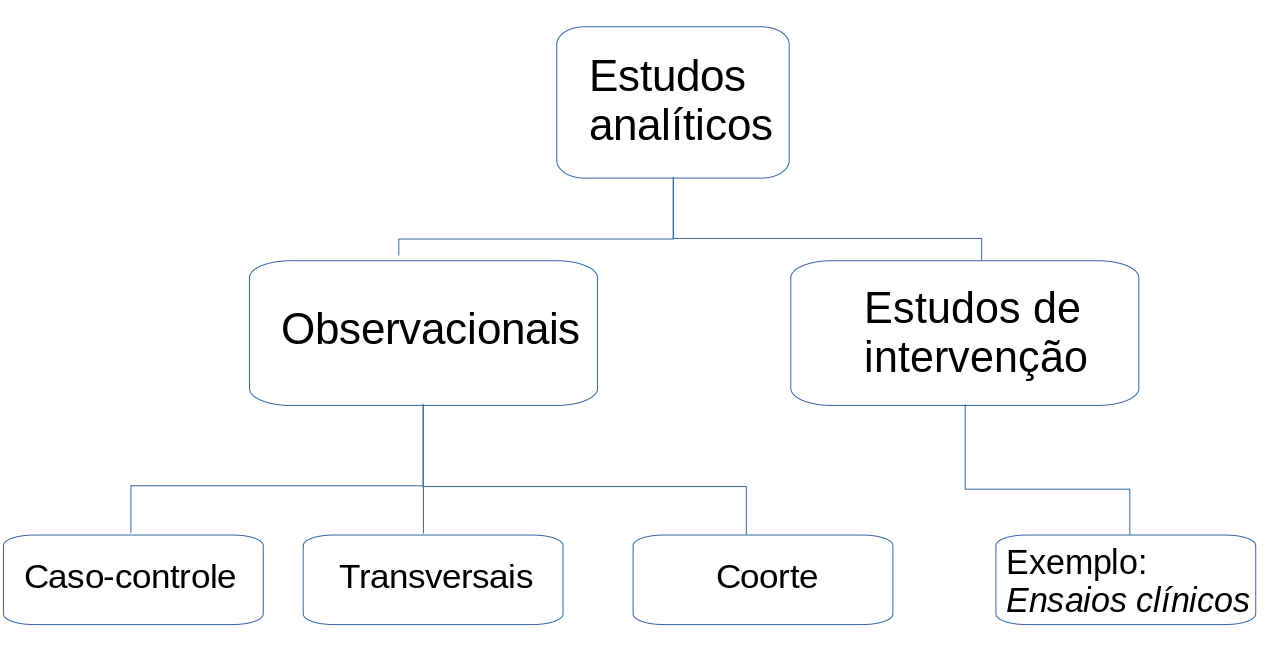
\includegraphics[width=0.9\linewidth]{figs/desenho_estudos} \end{center}
\end{frame}

\setbeamercovered{transparent}
\begin{frame}
\frametitle{Estudos caso-controles}
De uma mesma população são selecionadas amostras de indivíduos portadores de uma condição (casos) e outra de indivíduos não portadores (controle). Se há maior frequencia de exposição a uma situação entre os indivíduos portadores, temos um indício de que a exposição está relacionada à condição de interesse.
\begin{center}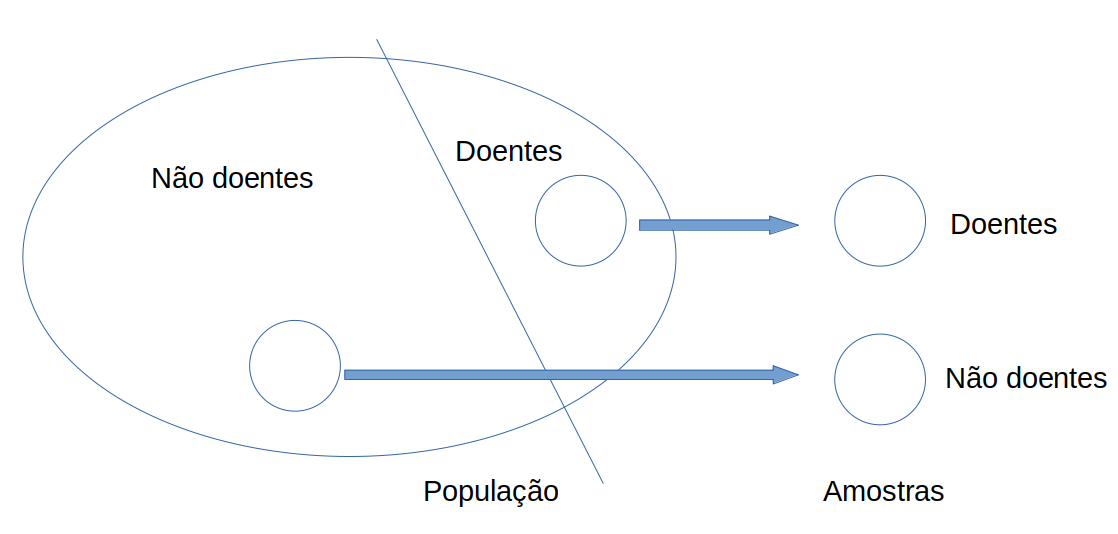
\includegraphics[width=0.8\linewidth]{figs/caso_controle} \end{center}
\end{frame}

\setbeamercovered{transparent}
\begin{frame}
\frametitle{Estudos transversais}
Seleciona-se uma amostra da população em questão, e posteriormente, verificamos quem é portador ou não da característica de interesse (por exemplo, doença). Objetiva-se obter uma estimativa da proporção de pessoas portadoras da característica. Como todas as informações da amostra são obtidas em um mesmo instante, pode ser difícil entender se a característica de interesse surgiu antes ou depois da exposição.
\begin{center}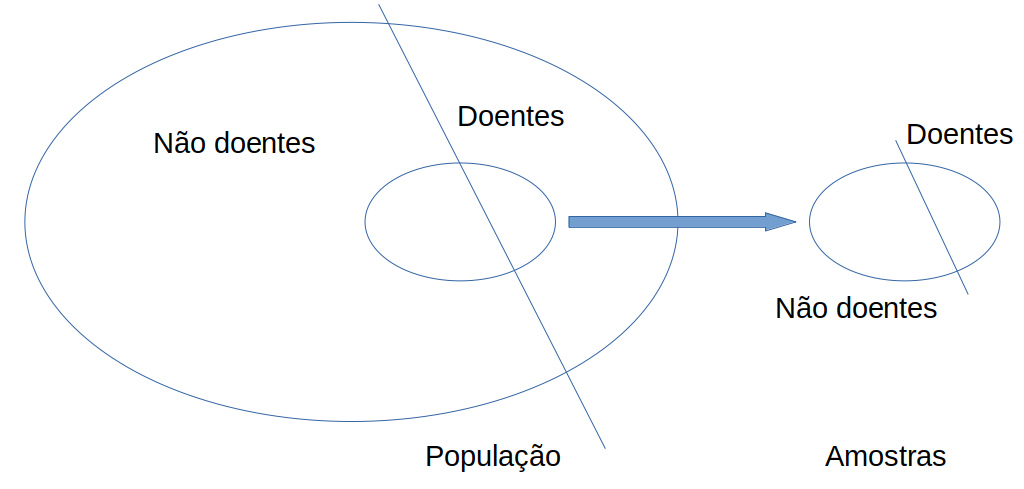
\includegraphics[width=0.8\linewidth]{figs/estudos_transversais} \end{center}
\end{frame}

\setbeamercovered{transparent}
\begin{frame}
\frametitle{Estudos de coorte}
Os indivíduos amostados são classificados como expostos ou não a uma situação que pode (ou não) ocasionar um evento específico (como uma doença). Esses individuos são acompanhados durante um período, e se ocorrer um mais eventos entre indivíduos expostos, temos evidências que a exposição pode ocasionar aquele evento.
\begin{center}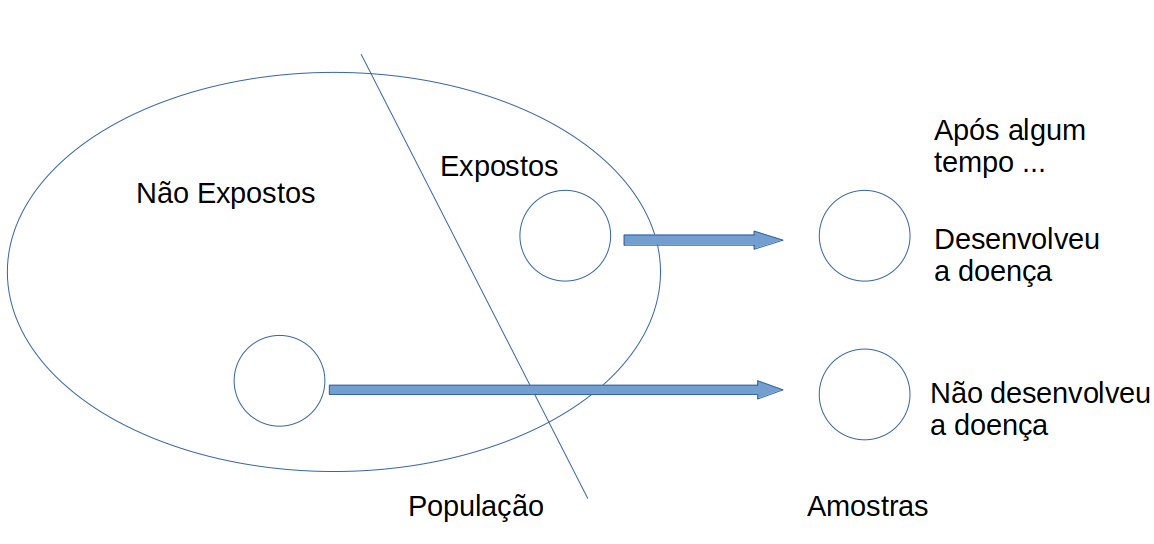
\includegraphics[width=0.8\linewidth]{figs/coorte} \end{center}
\end{frame}

\setbeamercovered{transparent}
\begin{frame}
\frametitle{Estudos de intervenção}
Objetiva-se administrar um tipo de intervenção capaz de alterar algum aspecto dos indivíduos, como o estado de saúde. Os estudos podem ser caracterizados como profiláticos ou terapêuticos. Um tipo de intervenção comum é o ensaio controlado aleatorizado, em que os indivíduos elegiveis ao estudo são divididos ao acaso em dois ou mais grupos. O grupo que não recebe a intervenção, ou tratamento, é geralmente denominado grupo controle. Outro tipo de estudo de intervenção é chamado de ensaio de não superioridade, cujo objetivo é entender se a intervenção estudada é tão benéfica quanto outra tradicionalmente utillizada no tratamento de uma condição.

\blfootnote{\url{https://forms.gle/64RgrBubuHih9NYf7}}
\end{frame}

\setbeamercovered{transparent}
\begin{frame}
\frametitle{Planejamento da coleta de dados}
\Fontvi

  \uncover<1->{
  Definição do experimento

  \begin{itemize}
  \item
    Variáveis respostas/interesse.
  \item
    Variáveis de controle (o que afeta a resposta?).
  \item
    Desenho do experimento e randomização. \\~\\
  \end{itemize}
  }

  \uncover<2->{
  Coleta de dados por amostragem

  \begin{itemize}
  \item
    Definição da população e característica de interesse.
  \item
    Definição do plano amostral:

    \begin{itemize}
    \item
      Aleatória simples (com ou sem reposição) ou sistemática;
    \item
      Estratificada, por estratos da população (segundo uma
      característica);
    \item
      Conglomerados, por grupos de indivíduos da população
      (subpopulações);
    \item
      Amostragem complexa (combina anteriores). \\~\\
    \end{itemize}
    \end{itemize}
   }

\end{frame}


\setbeamercovered{transparent}
\begin{frame}
\frametitle{Divisões básicas da estatística}

  Divisões essenciais em Estatística e seus principais objetivos. \\~\\

  \uncover<1->{
    Estatística descritiva ou exploratória:

    \begin{itemize}
    \item
      Consistência dos dados e interpretações iniciais.
    \item
      Visualização dos dados e relações entre variáveis. \\~\\
    \end{itemize}
  }
  \uncover<2->{
    Probabilidade:

    \begin{itemize}
    \item
      Fornece ferramentas para lidar/quantificar incerteza. \\~\\
    \end{itemize}
  }
  \uncover<3->{
    Inferência estatística:

    \begin{itemize}
    \item
      Estimação de quantidades desconhecidas.
    \item
      Formular e testar hipóteses.
    \item
      Extrapolar para a população resultados obtidos na amostra. \\~\\
      \url{https://forms.gle/rFGBJ9B6KYowaoJ6A}
    \end{itemize}
  }
\end{frame}

\setbeamercovered{transparent}
\begin{frame}
\frametitle{Divisões básicas da estatística}

\begin{center}\includegraphics[width=1.0\linewidth]{figs/organograma_estatistica} \end{center}
\blfootnote{\url{http://www.leg.ufpr.br/}}
\end{frame}

\section{Análise exploratória de dados}
\setbeamercovered{transparent}
\begin{frame}
\frametitle{Exemplo}

Pesquisa foi realizada com alunos. Variáveis:

\begin{itemize}
\item
  \textbf{Id}: identificação do aluno; \textbf{Turma}: A ou B;
\item
  \textbf{Sexo}: feminino (F) ou masculino (M);
\item
  \textbf{Idade}: em anos; \textbf{Alt}: altura em metros;
\item
  \textbf{Peso}: em quilogramas; \textbf{Filhos}: nº de filhos na
  família;
\item
  \textbf{Fuma}: hábito de fumar: sim (S) ou não (N);
\item
  \textbf{Toler}: tolerância ao cigarro: (I) indiferente; (P) incomoda
  pouco; (M) incomoda muito;
\item
  \textbf{Exerc.}: horas de atividade física, por semana;
\item
  \textbf{Cine}: nº. de vezes que vai ao cinema por semana;
\item
  \textbf{OpCine}: opinião a respeito das salas de cinema na cidade: (B)
  regular a boa; (M) muito boa;
\item
  \textbf{TV}: horas gastas assistindo TV, por semana;
\item
  \textbf{OpTV}: opinião a respeito da qualidade da programação na TV:
  (R) ruim; (M) média; (B) boa; (N) não sabe.
\end{itemize}
\end{frame}

\setbeamercovered{transparent}
\begin{frame}
\frametitle{Organização dos dados}

\begin{itemize}
\item
  A partir de um conjunto de dados coletado, a questão é:

  \begin{itemize}
  \item
    Como extrair informações a respeito de uma ou mais características
    de interesse?
  \end{itemize}
\item
  Basicamente temos duas opções:

  \begin{itemize}
  \item
    Tabelas de frequência;
  \item
    Gráficos.
  \end{itemize}
\item
  O importante é levar em consideração a \textbf{natureza dos dados}.
\end{itemize}
\end{frame}


\setbeamercovered{transparent}
\begin{frame}
\frametitle{Tipos de variáveis}

\begin{center}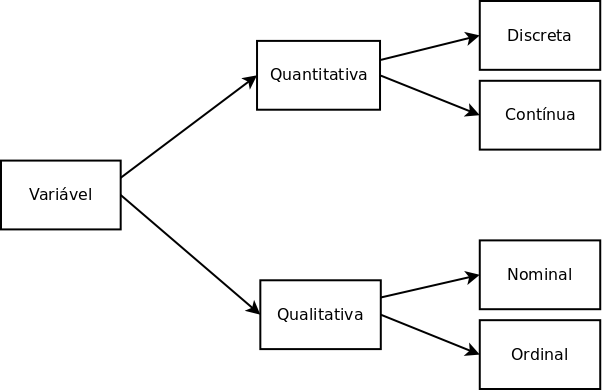
\includegraphics[width=0.85\linewidth]{figs/classificacao_variaveis} \end{center}
\blfootnote{\url{https://forms.gle/A3ENQCxDKpNDkNeR6}}
\end{frame}

\setbeamercovered{transparent}
\begin{frame}
\frametitle{Organização de Dados}

\begin{itemize}
\item
  Uma típica \textbf{tabela de dados brutos} contém:

  \begin{itemize}
  \item
    Variáveis (características, medições, etc) nas colunas.
  \item
    Sujeito (indivíduo, objetos, etc) nas linhas.
  \end{itemize}
\end{itemize}

\comment{

\begin{verbatim}
 Id Turma Sexo Idade  Alt Peso Filhos Fuma Toler Exerc Cine OpCine TV OpTV
  1     A    F    17 1.60 60.5      2  NAO     P     0    1      B 16    R
  2     A    F    18 1.69 55.0      1  NAO     M     0    1      B  7    R
  3     A    M    18 1.85 72.8      2  NAO     P     5    2      M 15    R
  4     A    M    25 1.85 80.9      2  NAO     P     5    2      B 20    R
  5     A    F    19 1.58 55.0      1  NAO     M     2    2      B  5    R
  6     A    M    19 1.76 60.0      3  NAO     M     2    1      B  2    R
\end{verbatim}
}

\begin{itemize}
\item
  Tipos de variáveis:

  \begin{itemize}
  \item
    Qualitativa nominal: Turma, Sexo, Fuma.
  \item
    Qualitativa ordinal: Toler, OpCine, OpTV.
  \item
    Quantitativa discreta: Idade, Filhos, Exerc, Cine, TV.
  \item
    Quantitativa contínua: Alt, Peso.
  \end{itemize}
\end{itemize}
\end{frame}


\setbeamercovered{transparent}
\begin{frame}
\frametitle{Tabelas de frequência}

\begin{itemize}
\item
  A tabela de dados brutos pode ser muito longa, portanto será difícil
  extrair alguma informação.
\item
  As \textbf{tabelas de frequência} ajudam a resumir a informação da
  variável de interesse.
\item
  Vamos usar 3 tipos de frequência:

  \begin{itemize}
  \item
    Frequência \textbf{absoluta}: contagem de cada valor observado.
    Representado por \(n_i\) o número de indivíduos com a característica
    \(i\).
  \item
    Frequência \textbf{relativa}: número de indivíduos com a
    característica \(i\) dividido pelo total de indivíduos \(n\), ou
    seja \(f_i = \frac{n_i}{n}\).
  \item
    Frequência \textbf{acumulada}: frequência (absoluta ou relativa)
    acumulada até um certo valor, obtida pela soma das frequências de
    todos os valores da variável, menores ou iguais ao valor
    considerado.
  \end{itemize}
\end{itemize}
\end{frame}

\setbeamercovered{transparent}
\begin{frame}
\frametitle{Tabela de frequência - qualitativa nominal}

\begin{itemize}
\item
  Considerando a variável \texttt{Sexo}
\end{itemize}

\begin{table}[ht]
\centering
\begin{tabular}{rrr}
  \hline
 & $n_i$ & $f_i$ \\ 
  \hline
F & 37 & 0.74 \\ 
  M & 13 & 0.26 \\ 
   \hline
Sum & 50 & 1.00 \\ 
   \hline
\end{tabular}
\end{table}

\begin{itemize}
\item
  Neste caso não faz sentido usar frequência acumulada.
\end{itemize}
\end{frame}

\setbeamercovered{transparent}
\begin{frame}
\frametitle{Tabela de frequência - qualitativa ordinal}

\begin{itemize}
\item
  Considerando a variável \texttt{OpTV}
\end{itemize}

\begin{table}[ht]
\centering
\begin{tabular}{rrrr}
  \hline
 & $n_i$ & $f_i$ & $f_{ac}$ \\ 
  \hline
R & 39 & 0.78 & 0.78 \\ 
  M & 1 & 0.02 & 0.80 \\ 
  B & 3 & 0.06 & 0.86 \\ 
  N & 7 & 0.14 & 1.00 \\ 
   \hline
Sum & 50 & 1.00 &  \\ 
   \hline
\end{tabular}
\end{table}
\end{frame}

\setbeamercovered{transparent}
\begin{frame}
\frametitle{Tabela de frequência - quantitativa discreta}

\begin{itemize}
\item
  Considerando a variável \texttt{Idade}
\end{itemize}

\begin{table}[ht]
\centering
\begin{tabular}{rrrr}
  \hline
 & $n_i$ & $f_i$ & $f_{ac}$ \\ 
  \hline
17 & 9 & 0.18 & 0.18 \\ 
  18 & 22 & 0.44 & 0.62 \\ 
  19 & 7 & 0.14 & 0.76 \\ 
  20 & 4 & 0.08 & 0.84 \\ 
  21 & 3 & 0.06 & 0.90 \\ 
  22 & 0 & 0.00 & 0.90 \\ 
  23 & 2 & 0.04 & 0.94 \\ 
  24 & 1 & 0.02 & 0.96 \\ 
  25 & 2 & 0.04 & 1.00 \\ 
   \hline
Sum & 50 & 1.00 &  \\ 
   \hline
\end{tabular}
\end{table}
\end{frame}

\setbeamercovered{transparent}
\begin{frame}
\frametitle{Tabela de frequência - quantitativa contínua}

\begin{itemize}
\item
  No caso de quantitativas contínuas não faz sentido contar cada valor
  pois podem existir muitos (potencialmente infinito).
\item
  A solução é criar \textbf{classes} ou \textbf{faixas de valores}, e
  contar o número de ocorrências dentro destas classes.
\item
  Para definir as classes:

  \begin{itemize}
  \item
    Defina a amplitude da classe, de maneira que se obtenham de 5 a 8
    classes (de mesma amplitude).
  \item
    Identifique os valores máximo e mínimo da variável e construa as
    classes de maneira que inclua todos os valores.
  \end{itemize}
\item
  As classes de valores podem seguir um dos formatos:
\end{itemize}

\comment{
\begin{longtable}[]{@{}llll@{}}
\toprule
Classe & Notação & Denominação & Resultado\tabularnewline
\midrule
\endhead
\([a,b)\) & \(a \vdash b\) & Fechado em a, aberto em b & Inclui a, não
inclui b\tabularnewline
\((a,b]\) & \(a \dashv b\) & Aberto em a, fechado em b & Não inclui a,
inclui b\tabularnewline
\bottomrule
\end{longtable}
}
\end{frame}

\setbeamercovered{transparent}
\begin{frame}
\frametitle{Tabela de frequência - quantitativa contínua}

\begin{itemize}
\item
  Considerando a variável \texttt{Peso}

  \begin{itemize}
  \item
    Foram construídas 6 classes de amplitude 10.
  \item
    As classes são do tipo \([a,b)\) ou \(a \vdash b\).
  \end{itemize}
\end{itemize}


\begin{table}[ht]
\centering
\begin{tabular}{rrrr}
  \hline
 & $n_i$ & $f_i$ & $f_{ac}$ \\ 
  \hline
$[40,50)$ & 8 & 0.16 & 0.16 \\ 
  $[50,60)$ & 22 & 0.44 & 0.60 \\ 
  $[60,70)$ & 8 & 0.16 & 0.76 \\ 
  $[70,80)$ & 6 & 0.12 & 0.88 \\ 
  $[80,90)$ & 5 & 0.10 & 0.98 \\ 
  $[90,100)$ & 1 & 0.02 & 1.00 \\ 
   \hline
$Sum$ & 50 & 1.00 &  \\ 
   \hline
\end{tabular}
\end{table}
\end{frame}


\setbeamercovered{transparent}
\begin{frame}
\frametitle{Tabela de frequência - quantitativa discreta (muitos
valores)}

\begin{itemize}
\item
  Considerando a variável \texttt{TV}.
\item
  Apesar de ser discreta, o número de valores únicos é muito grande e
  não seria útil contar as frequências de cada valor.
\item
  Neste caso, utiliza-se o mesmo procedimento usado para quantitativas
  contínuas

  \begin{itemize}
  \item
    Foram construídas 6 classes de amplitude 6\footnote{\textbf{Obs.}:
      no livro a tabela tem 5 classes, pois a última tem comprimento 12}.
  \end{itemize}
\end{itemize}

\begin{table}[ht]
\centering
\begin{tabular}{rrrr}
  \hline
 & $n_i$ & $f_i$ & $f_{ac}$ \\ 
  \hline
$[0,6)$ & 14 & 0.28 & 0.28 \\ 
  $[6,12)$ & 17 & 0.34 & 0.62 \\ 
  $[12,18)$ & 11 & 0.22 & 0.84 \\ 
  $[18,24)$ & 4 & 0.08 & 0.92 \\ 
  $[24,30)$ & 3 & 0.06 & 0.98 \\ 
  $[30,36)$ & 1 & 0.02 & 1.00 \\ 
   \hline
$Sum$ & 50 & 1.00 &  \\ 
   \hline
\end{tabular}
\end{table}
\end{frame}

\setbeamercovered{transparent}
\begin{frame}
\frametitle{Representação gráfica}

\begin{itemize}
\item
  Podemos visualizar as tabelas através de gráficos.
\item
  Existe um tipo de gráfico adequado para cada tipo de variável.
\item
  Cuidado deve ser tomado com representações visuais pois um gráfico
  desproporcional pode gerar interpretações distorcidas.
\item
  As principais representações gráficas são:

  \begin{itemize}
  \item
    Diagrama circular (setores ou ``pizza'');
  \item
    Gráfico de barras;
  \item
    Histogramas;
  \item
    Boxplots.
  \end{itemize}
\end{itemize}
\end{frame}

\setbeamercovered{transparent}
\begin{frame}
\frametitle{Diagrama circular}

\begin{itemize}
\item
  Adequado para variáveis qualitativas nominal e ordinal.
\end{itemize}


\begin{center}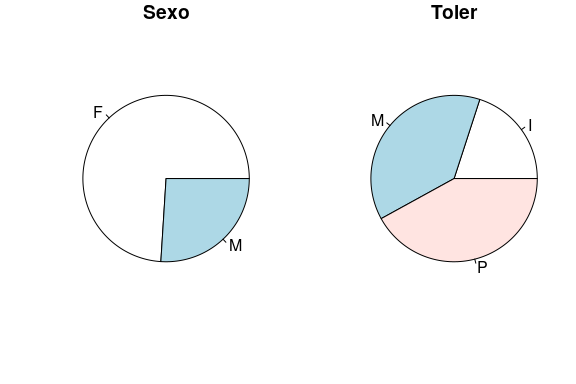
\includegraphics[width=0.7\linewidth]{figs/pie_chart} \end{center}


\begin{itemize}
\item
  O uso deste tipo de gráfico deve ser evitado, pois pode ser de difícil
  interpretação.
\end{itemize}
\end{frame}

\setbeamercovered{transparent}
\begin{frame}
\frametitle{Gráfico de barras}

\begin{itemize}
\item
  Adequado para variáveis qualitativas nominal/ordinal e quantitativa
  discreta (poucos valores distintos).
\item
  Podem ser usadas as frequências absolutas ou relativas.
\end{itemize}

\begin{center}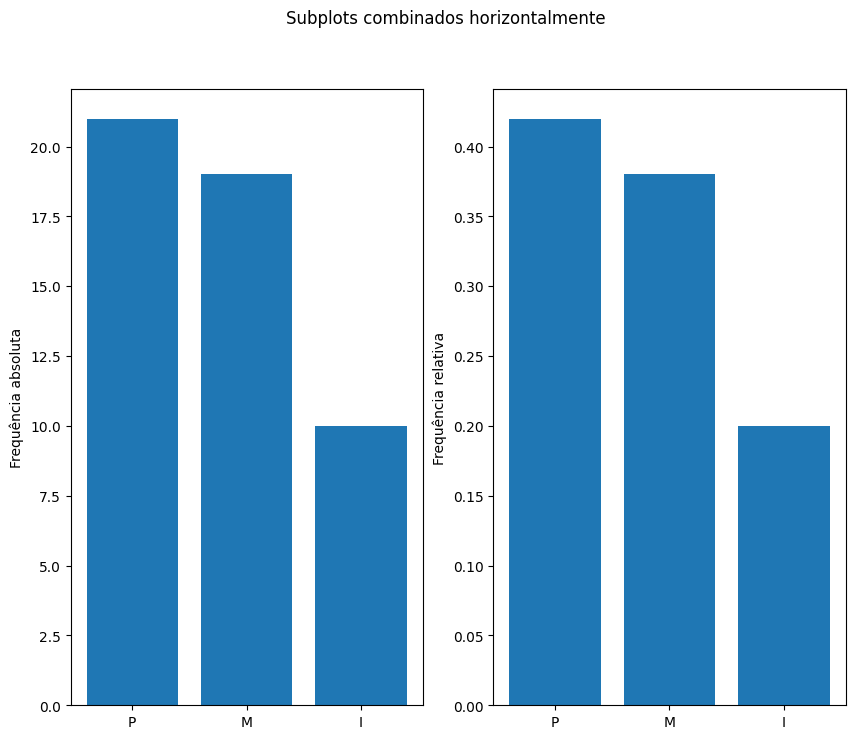
\includegraphics[width=0.5\linewidth]{figs/bar_plot2.png} \end{center}
\end{frame}

\setbeamercovered{transparent}
\begin{frame}
\frametitle{Histograma}

\begin{itemize}
\item
  Adequado para quantitativa contínua.
\end{itemize}

\begin{center}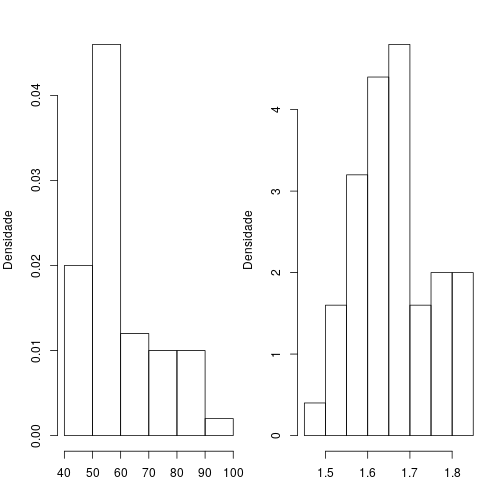
\includegraphics[width=0.4\linewidth]{figs/histogram} \end{center}

\begin{itemize}
\item
  Altura de cada retângulo é a densidade definida pelo quociente da área
  pela amplitude da faixa, \(h = \frac{f_i}{AMP}\).
\end{itemize}
\end{frame}

\setbeamercovered{transparent}
\begin{frame}
\frametitle{Tipos de assimetria}

\begin{center}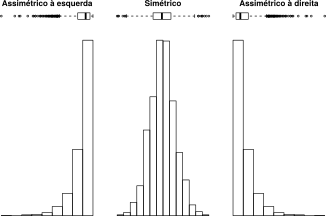
\includegraphics[width=0.6\linewidth]{figs/hist_simetria} \end{center}
\end{frame}

\setbeamercovered{transparent}
\begin{frame}
\frametitle{Mediana e quartis}

\begin{itemize}
\item
  \textbf{Mediana}: valor da variável que divide o conjunto de dados
  ordenado em dois subgrupos de mesmo tamanho.
\item
  \textbf{Quartis}: valores da variável que divide o conjunto de dados
  ordenados em quatro subgrupos de mesmo tamanho.
\item
  \textbf{Posição} dos quartis:

  \begin{itemize}
  \item
    \(Q_1 = 0.25 \cdot (N+1)\) e arredonde.
  \item
    \(Q_2 =\) média dos valores nas posições \((N/2)\) e \((N/2)+1\) se
    N par e \(Q_2 = (N+1)/2\) se N ímpar.
  \item
    \(Q_3 = 0.75 \cdot (N+1)\) e arredonde.
  \end{itemize}
\item
  Exemplo: Conside o conjunto de dados: \(8.43(1)\), \(8.65(2)\),
  \(9.96(3)\), \(10.91(6)\), \(10.46(4)\) e \(10.83(5)\).

  \begin{itemize}
  \item
    \(Q_1 = 0.25 \cdot 7 = 1.75 \approx 2\), ou seja \(8.65\).
  \item
    \(Q_2 =\) média dos valores nas posições \(3\) e \(4\), ou seja,
    \((9.96 +  10.46 )/2 = 10.21\).
  \item
    \(Q_3 = 0.75 \cdot 7 = 5.25 \approx 5\), ou seja, \(10.83\).
  \end{itemize}
\end{itemize}
\end{frame}

\setbeamercovered{transparent}
\begin{frame}
\frametitle{Boxplot}

\begin{itemize}
\item
  Adequado para quantitativa contínua.
\item
  Pode ser usado também para quantitative discreta com muitos valores.
\end{itemize}

\begin{center}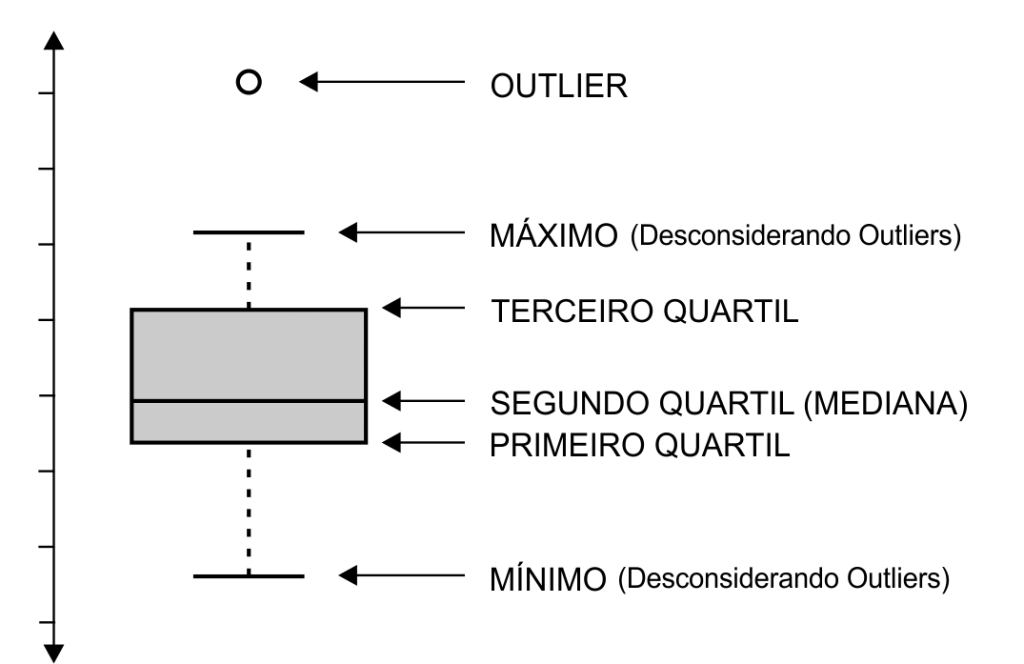
\includegraphics[width=0.6\linewidth]{figs/boxplot} \end{center}
\end{frame}

\setbeamercovered{transparent}
\begin{frame}
\frametitle{Boxplots}

\begin{itemize}
\item
  Excelente para explorar relações entre qualitativas e contínuas.
\end{itemize}

\begin{center}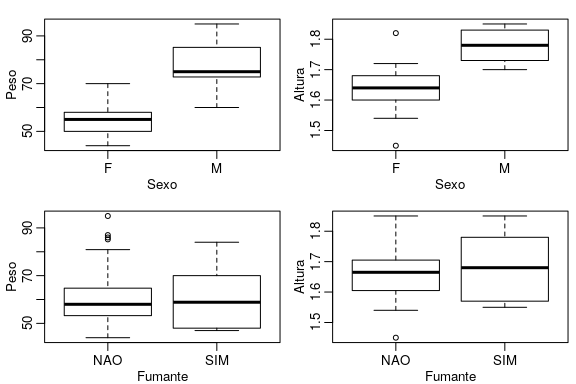
\includegraphics[width=0.7\linewidth]{figs/bx.png} \end{center}
\end{frame}

\setbeamercovered{transparent}
\begin{frame}
\frametitle{Diagrama de dispersão}

\begin{itemize}
\item
  Adequado para explorar a relação entre variáveis quantitativas.
\end{itemize}

\begin{center}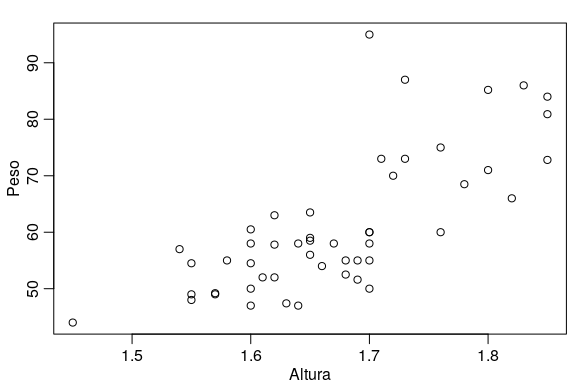
\includegraphics[width=0.8\linewidth]{figs/dispersao} \end{center}
\end{frame}

\setbeamercovered{transparent}
\begin{frame}
\frametitle{Diagrama de dispersão}

\begin{itemize}
\item
  Exemplos de comportamentos do diagrama de dispersão.
\end{itemize}

\begin{center}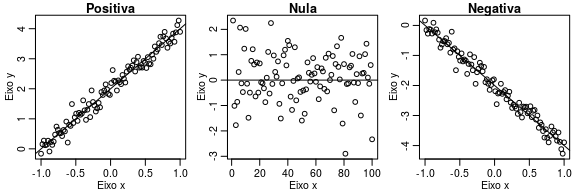
\includegraphics[width=1\linewidth]{figs/multi_dispersao} \end{center}
\end{frame}

\setbeamercovered{transparent}
\begin{frame}
\frametitle{Diagrama de dispersão}

\begin{itemize}
\item
  Formas não lineares.
\end{itemize}

\begin{center}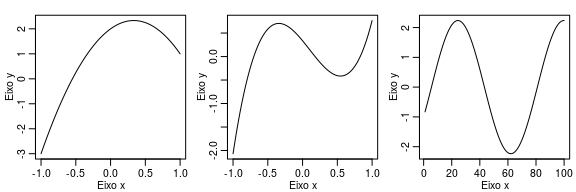
\includegraphics[width=1\linewidth]{figs/multi_lines} \end{center}
\end{frame}

\setbeamercovered{transparent}
\begin{frame}
\frametitle{Gráfico de mosaico}

\begin{itemize}
\item
  Adequado para explorar a relação entre variáveis qualitativas
  (nominais ou ordinais).
\end{itemize}

\begin{center}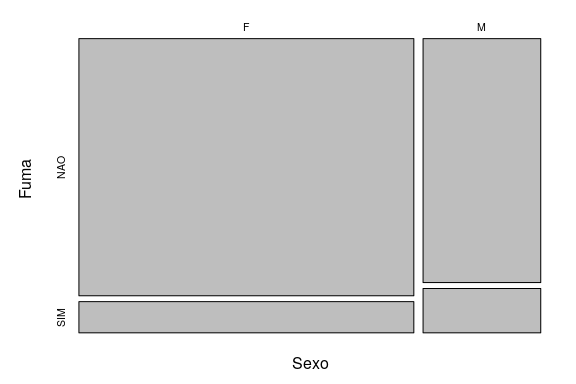
\includegraphics[width=0.6\linewidth]{figs/mosaico} \end{center}
\blfootnote{\url{https://plotly.com/python/}}
\end{frame}

\subsubsection{Resumo}

\setbeamercovered{transparent}
\begin{frame}
\frametitle{Resumo}
\begin{itemize}
\item
  Qualitativa nominal ou ordinal

  \begin{itemize}
  \item
    Gráfico de setores.
  \item
    Gráfico de barras.
  \end{itemize}
\item
  Quantitativa discreta

  \begin{itemize}
  \item
    Gráfico de barras (poucos valores).
  \item
    Histograma ou boxplot (muitos valores).
  \end{itemize}
\item
  Quantitativas contínuas

  \begin{itemize}
  \item
    Histograma ou boxplot.
  \end{itemize}
\item
  Explorando relações:

  \begin{itemize}
  \item
    Quantivativa vs Quantitativa: Diagrama de dispersão.
  \item
    Qualitativa vs Quantitativa: Boxplots.
  \item
    Qualitativa vs Qualitativa: Gráfico de mosaico.
  \end{itemize}
\end{itemize}
\end{frame}

\setbeamercovered{transparent}
\begin{frame}
\frametitle{Exercícios recomendados}

\begin{itemize}
\item
  Seção 1.1: Ex. 2 e 3.
\item
  Seção 1.2: Ex. 4.
\item
  Seção 1.4: Ex. 1, 3, 5, 9, 19 e 21.
\end{itemize}
\end{frame}

\setbeamercovered{transparent}
\begin{frame}
\frametitle{Referências bibliográficas}
\printbibliography
\end{frame}

\end{document}